\chapter{Estado del arte}

En el presente capítulo se realizará un análisis completo de los conceptos clave abordados a lo largo del proyecto. En particular, 
se describen las técnicas, los dispositivos, las herramientas y el contexto general asociados a la navegación autónoma. Asimismo, 
se presta especial atención a los antecedentes y al estado actual de las soluciones propuestas en los últimos años, considerando tanto 
sus fundamentos teóricos como su aplicación práctica.

Asimismo, se revisan los enfoques más relevantes para la percepción del entorno, la estimación del movimiento y la evitación de obstáculos 
en escenarios interiores, con énfasis en las limitaciones impuestas por plataformas aéreas de pequeño tamaño. Esta revisión permite 
contextualizar las decisiones de diseño adoptadas en el sistema propuesto y justificar la selección de sensores, algoritmos y modelos 
empleados.

Finalmente, se establecen los criterios de comparación utilizados a lo largo del capítulo, incluyendo aspectos como la robustez frente a 
cambios de iluminación, el coste computacional, la latencia de ejecución y la precisión alcanzable en la estimación de profundidad y 
localización.

\section{Navegación autónoma de vehículos no tripulados}
    La navegación autónoma ha constituido una línea de investigación central en robótica desde sus orígenes. Entre los primeros hitos destaca 
    \textit{Shakey}~\cite{shakey}, desarrollado en el Stanford Research Institute (SRI) durante el periodo 1966--1972, considerado uno de los 
    primeros sistemas móviles capaces de percibir el entorno y planificar acciones de forma autónoma. Este trabajo demostró la viabilidad de 
    integrar sensórica básica con técnicas de razonamiento y planificación, sentando las bases de numerosos desarrollos posteriores.

    Un impulso relevante para el avance de la autonomía lo aportó la Agencia de Proyectos de Investigación Avanzados de Defensa (DARPA), 
    mediante la organización de competiciones que incentivaron el desarrollo y la maduración de sistemas autónomos en condiciones realistas. 
    En este contexto, el vehículo \textit{Stanley}~\cite{stanley}, desarrollado por la Universidad de Stanford, resultó vencedor del 
    DARPA Grand Challenge de 2005, mientras que \textit{Boss}~\cite{boss}, desarrollado por Carnegie Mellon University en colaboración con 
    General Motors, obtuvo un papel destacado en el DARPA Urban Challenge de 2007.

    La evolución posterior de estas iniciativas impulsó la consolidación de metodologías de percepción, localización, planificación y control 
    que, con distintas adaptaciones, han sido transferidas progresivamente a otros dominios, incluyendo los vehículos aéreos no tripulados.

    En los últimos años se han desarrollado soluciones prácticas aplicables a múltiples plataformas, incluyendo vehículos tipo Ackermann, 
    robots cuadrúpedos~\cite{spot-boston}, humanoides~\cite{atlas-boston} e, incluso, sistemas de robótica blanda. En este último ámbito, se 
    han propuesto robots con morfologías no convencionales, como los robots de tipo serpiente~\cite{snake-like-robot}, capaces de operar en 
    entornos de geometría compleja y de difícil acceso, lo que ha ampliado el alcance de la navegación autónoma hacia escenarios anteriormente 
    inaccesibles.

    En el caso concreto de los UAV, la navegación autónoma plantea retos adicionales derivados de la necesidad de mantener la estabilidad en 
    vuelo, operar con restricciones estrictas de peso y consumo energético, y reaccionar con latencias reducidas ante obstáculos y 
    perturbaciones. Por este motivo, el diseño de sistemas de navegación para plataformas aéreas suele priorizar soluciones ligeras y robustas, 
    en las que la percepción del entorno y la planificación de trayectorias deben ejecutarse en tiempo real con recursos computacionales 
    limitados.


\subsection{Navegación autónoma en UAVs}

    La navegación autónoma en vehículos aéreos no tripulados ha constituido uno de los principales temas de investigación en los últimos años, 
    impulsada por su creciente adopción en sectores como la defensa, el transporte y la agricultura. En este contexto, la navegación se apoya 
    en técnicas clásicas de estimación del estado a partir de sensórica embarcada, destacando el uso de unidades de medida inercial (IMU) para 
    la estimación de actitud y estabilidad, así como el empleo de GNSS/GPS para la obtención de posición global cuando la señal se encuentra 
    disponible. Sin embargo, en entornos interiores o en escenarios con degradación de la señal GNSS, resulta necesario recurrir a estrategias 
    alternativas basadas en percepción, donde adquieren especial relevancia los sensores visuales y los sensores inerciales , así como la 
    fusión multisensor para incrementar la robustez y la precisión del sistema.

    En particular, la odometría visual-inercial (VIO) y otros esquemas de fusión permiten mitigar la deriva inherente de la estimación 
    puramente inercial, aunque persisten desafíos significativos asociados a la sensibilidad frente a variaciones de iluminación, oclusiones 
    y ambigüedad de escala, además de los requisitos computacionales necesarios para ejecutar métodos de filtrado u optimización en tiempo real. 
    Finalmente, el uso de técnicas de inteligencia artificial ha adquirido una relevancia creciente en este ámbito, al permitir mejorar la 
    percepción y la estimación de la odometría incluso con configuraciones sensoriales limitadas. No obstante, su usabilidad continúa 
    condicionada por las restricciones de cómputo~\cite{advancedments-uavs}.


\section{Arquitecturas de control}
    Uno de los avances más relevantes en el ámbito de la navegación autónoma ha sido el desarrollo de nuevas arquitecturas de control, 
    tanto en términos de planificación de trayectorias como en la incorporación de información sensorial alternativa. En cualquier caso la mayoría de los sistemas de 
    navegación comparten un marco conceptual común a nivel de sistema.

    \subsection{Marco teórico de control en la navegación autónoma}
    La complejidad inherente de la navegación autónoma, como ocurre en numerosas aplicaciones de robótica móvil, ha motivado que su estudio 
    y desarrollo se organicen en módulos de menor complejidad. Este enfoque modular permite abordar de forma separada los distintos 
    problemas. En términos generales, el objetivo es dotar al sistema de la capacidad de 
    adquirir información procedente de múltiples sensores y fusionarla de manera coherente, de modo que se obtenga una estimación única del 
    estado del vehículo, reflejando además, las incertidumbres de cada fuente de medida.

    En este contexto, la \textit{localización} constituye un concepto fundamental. Disponer de una estimación fiable de la posición y 
    orientación del vehículo resulta imprescindible para seguir una trayectoria o para alcanzar un objetivo determinado. 
    En ausencia de una referencia del estado actual, no es posible verificar el seguimiento correcto de la ruta ni determinar con 
    garantías si se ha alcanzado el destino.

    El \textit{mapeado}, aunque no es estrictamente necesario en todos los escenarios, desempeña un papel relevante en sistemas de 
    navegación que requieren persistencia y capacidad de replanteamiento. El uso de un mapa permite identificar zonas previamente 
    visitadas, detectar inconsistencias y recalcular rutas para mejorar la evitación de obstáculos o la eficiencia del desplazamiento.

    Finalmente, los conceptos de \textit{planificación} y \textit{control} completan el marco teórico. El planificador global suele operar 
    a baja frecuencia y tiene como finalidad calcular una ruta, es decir, una secuencia de puntos o referencias entre el origen y el 
    destino, teniendo en cuenta la información disponible del entorno. Por el contrario, el planificador local o controlador opera a mayor frecuencia y 
    transforma dichas referencias en comandos de movimiento adecuados para el vehículo, ajustándolos en tiempo real en función de la 
    estimación del estado y de la información sensorial disponible. En la Figura~\ref{fig:control_theory_autnav} se representa una 
    arquitectura básica que resume estas relaciones funcionales.

    \begin{figure}[H]
    	\ffigbox[\FBwidth] {
            \caption[Arquitectura básica de control en navegación autónoma]{Arquitectura básica de control en navegación autónoma.}
            \label{fig:control_theory_autnav}
    	}
    	{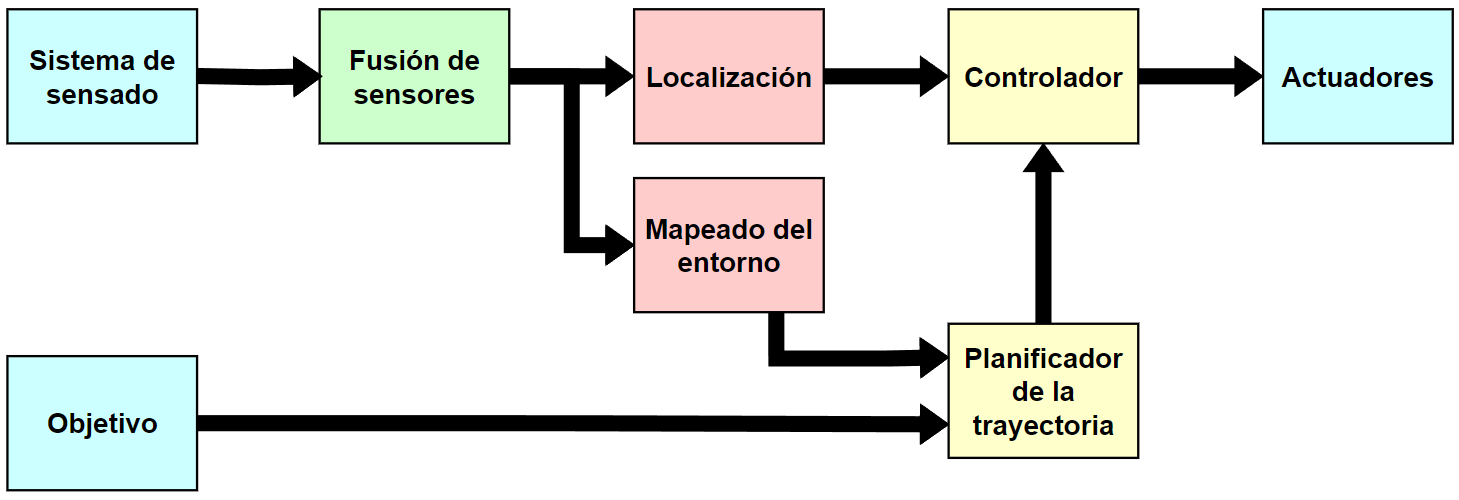
\includegraphics[scale=0.35]{images/control_theory_autnav.png}}
    \end{figure}


    \subsection{Planificadores globales y controladores}
    En las arquitecturas de navegación autónoma se distingue habitualmente entre \textit{planificación} y \textit{control}, dado que ambos
    procesos operan en escalas temporales distintas y persiguen objetivos complementarios. La planificación se encarga de generar una solución
    factible que conecte un estado inicial con un objetivo, imponiendo restricciones geométricas y de seguridad. Y por otro lado, el control
    ejecuta dicha solución en el sistema físico, transformando referencias en comandos actuables y compensando perturbaciones y la presencia de obstáculos.

    \subsubsection*{Planificadores}
    Los planificadores proporcionan una solución que permite que un vehículo navegue de forma segura en el espacio, dada una \textit{pose}
    inicial, un objetivo y un conjunto de restricciones (radio máximo de giro, modelo de movimiento, penalizaciones por cambios de trayectoria,
    heurística, entre otras). En función de los requisitos de la aplicación existen múltiples algoritmos y variantes, cada uno con ventajas y
    limitaciones. El tiempo de cálculo suele ser elevado, por lo que, en general, se ejecutan de manera previa al movimiento del robot o a una
    frecuencia reducida.

    Entre los métodos clásicos destaca el algoritmo de \textit{Dijkstra}, basado en grafos, que explora de forma exhaustiva y garantiza el
    camino de coste mínimo a cambio de un coste computacional elevado en espacios discretizados de gran tamaño. El algoritmo \textit{A*} puede
    entenderse como una extensión de Dijkstra que introduce una heurística para guiar la búsqueda, manteniendo la optimalidad bajo condiciones
    adecuadas y reduciendo el tiempo de cálculo en la práctica. Por su parte, variantes como \textit{D*} (y \textit{D* Lite}) están diseñadas
    para replanificar de forma eficiente ante cambios en el mapa, mientras que métodos como \textit{SMA*} limitan el consumo de memoria a costa
    de posibles reexpansiones. Finalmente, en espacios continuos o de alta dimensionalidad son frecuentes los planificadores basados en muestreo,
    como \textit{RRT} y \textit{RRT*}, mientras que algoritmos como \textit{DWA} se emplean habitualmente como planificadores locales al generar
    comandos de velocidad en tiempo real.

    En la Tabla~\ref{tab:planners_summary} se recogen, de forma comparativa, algunas ventajas y desventajas de los métodos más utilizados.

    \begin{table}[H]
        % \centering
        
        % \ttabbox
        {\caption{Tabla comparativa de planificadores para la navegación autónoma}
        \label{tab:planners_summary}}
        {%
        \begin{tabularx}{0.896\textwidth}{|c|c|c|}
            \hline
            \textbf{Método} & \textbf{Ventajas} & \textbf{Desventajas} \\
            \hline
            Dijkstra & Coste mínimo. & Alto coste computacional. \\
            \hline
            A* & Más eficiente que Dijkstra. & Dependencia de la heurística. \\
            \hline
            D* & Replanificación eficiente. & Mayor complejidad. \\
            \hline
            RRT & Eficiente en alta dimensionalidad. & Trayectoria subóptima. \\
            \hline
            RRT* & Converge asintóticamente. & Mayor tiempo de cómputo. \\
            \hline
            DWA & Respeta restricciones cinemáticas. & Propenso a mínimos locales. \\
            \hline
            SMA* & A* con memoria acotada. & Puede reexpandir nodos. \\
            \hline
            \multicolumn{3}{l}{Fuente: elaboración propia.} \\
        \end{tabularx}%
        }
    \end{table}

    En la práctica, una arquitectura robusta combina un planificador global con un planificador local: el primero define una ruta de alto
    nivel y el segundo adapta el movimiento a las condiciones reales del entorno (obstáculos no mapeados o dinámicos), respetando las
    restricciones de seguridad y la dinámica del vehículo. A este componente local se le suele denominar \textit{controlador} o, en algunos
    enfoques, planificador local.

    \subsubsection*{Planificador local}
    El planificador local transforma la referencia (trayectoria, posición o velocidad deseada) en comandos para el sistema de propulsión y los
    actuadores. En robótica móvil se emplean controladores clásicos como PID o LQR, así como métodos específicos para el seguimiento de
    trayectorias y la evitación local, tales como \textit{Pure Pursuit},Figura~\ref{fig:purepursuit}, o los \textit{campos potenciales}. Asimismo, el control predictivo
    basado en modelo (MPC) permite incorporar restricciones explícitas y anticipar la evolución del sistema, a costa de un mayor coste de
    cómputo. De forma general, se emplean lazos internos a alta frecuencia para estabilizar la actitud y la dinámica rápida, y lazos externos a
    menor frecuencia para regular la posición y ejecutar la navegación.

    En la Tabla~\ref{tab:controllers_summary} se resumen ventajas y desventajas de algunos controladores ampliamente utilizados.

    \begin{table}[H]
        \ttabbox
        {\caption{Tabla comparativa de controladores para la navegación autónoma}
        \label{tab:controllers_summary}}
        {%
        \begin{tabularx}{0.942\textwidth}{|c|c|c|}
            \hline
            \textbf{Método} & \textbf{Ventajas} & \textbf{Desventajas} \\
            \hline
            PID & Implementación simple y robusta. & Sin restricciones explícitas. \\
            \hline
            LQR & Estabilidad y rendimiento. & Requiere un modelo linealizado. \\
            \hline
            MPC & Anticipa la evolución del sistema. & Dependencia del modelo. \\
            \hline
            PP & Seguimiento sencillo (\textit{look-ahead}). & Propenso a oscilar. \\
            \hline
            APF & Reacción local rápida. & Propenso a mínimos locales. \\
            \hline
            \multicolumn{3}{l}{Fuente: elaboración propia.} \\
        \end{tabularx}%
        }
    \end{table}

La selección de planificador y controlador depende del entorno, del nivel de incertidumbre y, especialmente, de las
restricciones computacionales y temporales del sistema objetivo.

\begin{figure}[H]
    \ffigbox[\FBwidth] {
        \caption[Ejemplo de control por Pure Pursuit]{Ejemplo de control mediante Pure Pursuit.}
        \label{fig:purepursuit}
    }
    {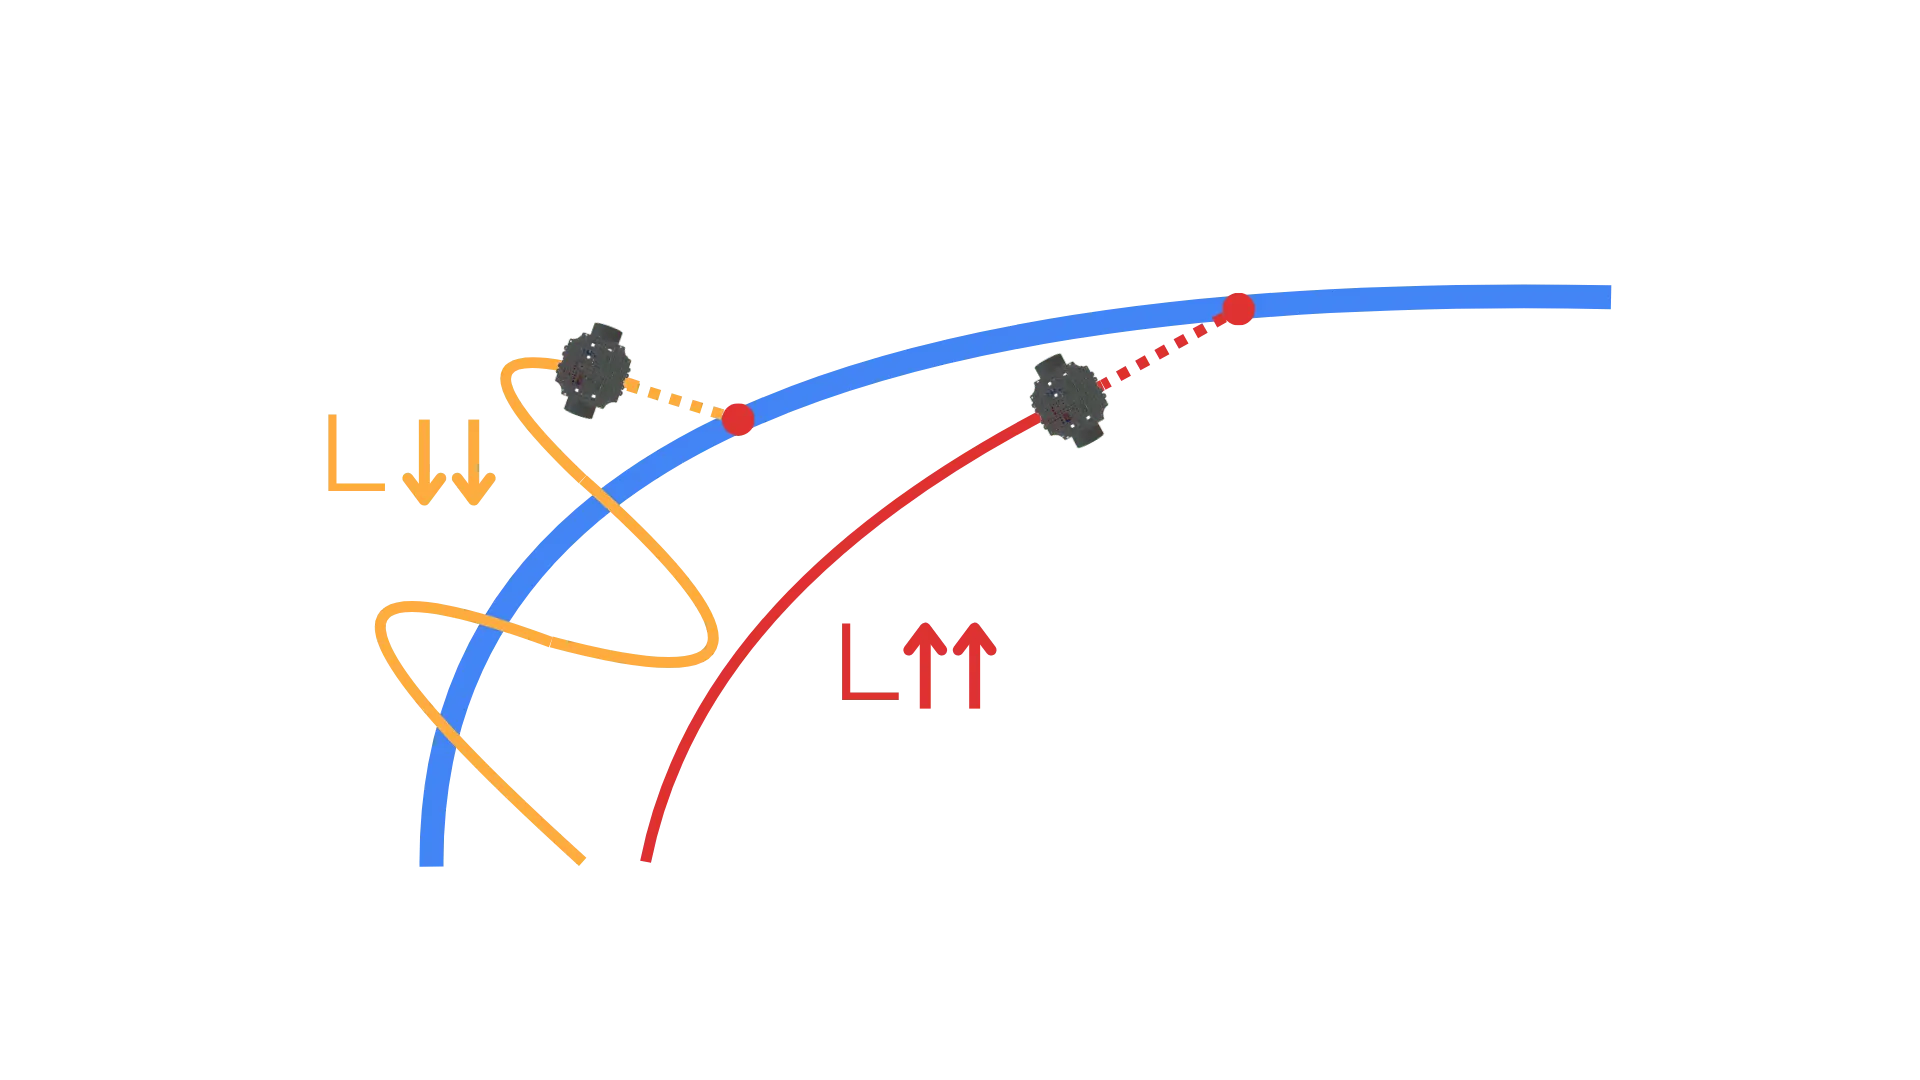
\includegraphics[scale=0.18]{images/pute_purpursuit.png}}
\end{figure}

    \subsection{Control mediante fusión visual-inercial(VI)}
    En el control aplicado a la navegación es habitual distinguir dos fuentes de estimación del estado con características complementarias. En
    primer lugar, se dispone de una fuente \textit{global} que proporciona una localización absoluta con alta precisión y sin deriva temporal,
    aunque normalmente a baja frecuencia (típicamente entre 1 y 10~Hz). En segundo lugar, se emplea una fuente \textit{local} u odométrica que,
    si bien acumula deriva con el tiempo, aporta estimaciones de manera continua a mayor frecuencia (del orden de 10 a 100~Hz), permitiendo
    mantener información del estado entre actualizaciones del sensor global. En la Figura~\ref{fig:loca-glob-loc} se ilustra este esquema: el
    localizador global corrige periódicamente la posición, mientras que, entre correcciones, la odometría estima el movimiento con un error que
    tiende a crecer con el tiempo. Mediante la fusión de ambas fuentes es posible obtener una estimación que combina localización absoluta sin
    deriva con disponibilidad continua a alta frecuencia.


    Generalmente, esta arquitectura se implementa mediante el uso de GNSS/GPS en exteriores o mediante Lidar y/o camaras 3D en itneriores como fuente global y el uso de
    encoders o IMUs como fuente odométrica. Estas son combinadas de manera estadisticas con un filtro, como puede ser un filtro de Kalma. En el caso de interés de este 
    trabajo, el localizador global suele basarse en información visual, mediante la extracción de
    características de una imagen 2D junto con la medida de una IMU a alta frecuencia para así, mantener una estimación continua del estado.
    \begin{figure}[H]
        \ffigbox[\FBwidth]{
            \caption[Esquema teórico de localización mediante odometría y sensor global]{Esquema teórico de localización mediante odometría y sensor global.}
            \label{fig:loca-glob-loc}
        }{
            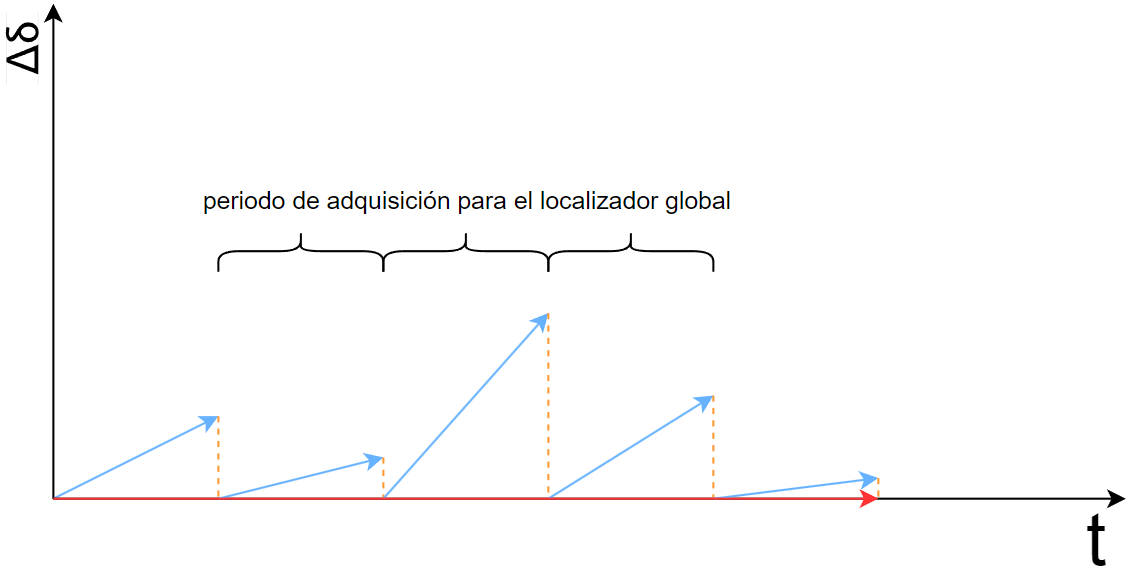
\includegraphics[scale=0.4]{images/localizador-global-local.png}
        }
    \end{figure}

    Desde la perspectiva del control, los sistemas VI se integran típicamente en una arquitectura jerárquica. En los lazos internos, el
    autopiloto estabiliza la actitud y regula la velocidad angular utilizando directamente la IMU, que ofrece tasas de actualización elevadas.
    En los lazos externos, la estimación de posición y velocidad proporcionada por VIO/VI-SLAM se emplea para generar referencias de movimiento
    (velocidades lineales, aceleraciones deseadas o puntos de paso) que guían el desplazamiento. Dado que la estimación visual puede estar
    limitada por la tasa de fotogramas, las condiciones de iluminación o la ausencia de textura, es habitual emplear fusión temporal para
    aprovechar simultáneamente la alta frecuencia de la IMU y la capacidad correctiva de la cámara.

    Un aspecto relevante en la navegación VI es la gestión de incertidumbre y latencia. La estimación visual suele introducir retardo de
    procesamiento. En consecuencia, el diseño del controlador debe considerar dichas latencias para evitar inestabilidades, por ejemplo mediante predicción del
    estado al tiempo actual, filtrado de medidas o reducción de la agresividad de maniobra cuando disminuye la confianza en la estimación. De
    forma análoga, el sistema debe contemplar condiciones adversas como cambios bruscos de iluminación, desenfoque por movimiento u oclusiones que pueden degradar la 
    calidad de la odometría. En tales casos, la IMU actúa como soporte.

    En aplicaciones prácticas, el enfoque VI condiciona también decisiones de diseño a nivel de percepción. La elección de cámara (\textit{global
    shutter} frente a \textit{rolling shutter}), la calibración intrínseca y extrínseca, la sincronización temporal entre cámara e IMU y el
    modelado adecuado de sesgos inerciales influyen de forma directa en la estabilidad del control. En particular, la sincronización resulta
    crítica: errores temporales pequeños pueden traducirse en estimaciones inconsistentes. Por ello, los
    sistemas VI robustos priorizan una cadena de adquisición bien caracterizada y procedimientos de calibración robustos.


    % \subsection{Mención honorífica, ROS}
    % ROS (\textit{Robot Operating System}) ha desempeñado un papel fundamental en la consolidación de arquitecturas modulares en robótica,
    % facilitando la reutilización de algoritmos y acelerando la integración de sistemas complejos. Su modelo basado en \textit{nodos} que
    % intercambian información mediante \textit{tópicos}, \textit{servicios} y \textit{acciones} permite desacoplar componentes de percepción,
    % localización, planificación y control. Esta separación favorece la mantenibilidad y permite sustituir módulos sin modificar el resto del
    % sistema, siempre que se conserven las interfaces, lo cual resulta especialmente valioso en proyectos de investigación y desarrollo donde
    % la iteración es constante.

    % Dentro de este ecosistema, Nav2 (Navigation2) representa una arquitectura versátil para navegación en ROS~2, diseñada para integrarse de
    % manera flexible con diferentes sensores, fuentes de localización y estrategias de planificación y control. Su estructura se apoya en un
    % conjunto de servidores especializados (\textit{planner server}, \textit{controller server}, \textit{behavior server}, entre otros),
    % conectados mediante \textit{actions} y gobernados por \textit{behavior trees}, lo que permite definir comportamientos complejos de forma
    % declarativa. Esta arquitectura facilita sustituir planificadores y controladores mediante plugins, ajustar parámetros sin alterar código y
    % adaptar el sistema a distintos requisitos de hardware o de entorno.

    % En consecuencia, ROS y, en particular, Nav2, han contribuido de forma notable a que la implementación de arquitecturas de navegación sea
    % más accesible y reproducible. La modularidad inherente reduce el esfuerzo de integración y permite centrar el desarrollo en componentes
    % específicos (por ejemplo, percepción o estimación de profundidad), manteniendo una infraestructura estable para la coordinación del sistema.
    \section{Localización (VIO)}
    La localización constituye uno de los bloques fundamentales en un sistema de navegación autónoma, ya que permite estimar la \textit{pose}
    del vehículo a partir de la información sensorial disponible. En el caso de plataformas aéreas, esta estimación debe
    obtenerse con baja latencia, suficiente precisión y un coste computacional compatible con las restricciones del sistema.

    En este contexto, la odometría visual-inercial (\textit{Visual-Inertial Odometry}, VIO) permite estimar el movimiento relativo del sensor
    combinando imágenes de una o varias cámaras con medidas proporcionadas por una unidad de medida inercial (IMU). A diferencia de un sistema
    SLAM completo, cuyo objetivo incluye la construcción y mantenimiento de un mapa global del entorno, un sistema VIO se centra principalmente
    en estimar de forma local y continua la trayectoria del vehículo respecto a un marco de referencia inicial. Por tanto, la salida principal
    del sistema es una estimación de posición, orientación y, en muchos casos, velocidad.

    Desde un punto de vista funcional, un sistema VIO suele estar formado por dos bloques principales. El primero es un \textit{front-end}
    visual, encargado de procesar las imágenes, detectar o seguir características y generar correspondencias temporales entre fotogramas. El
    segundo es un estimador de estado, que combina dichas observaciones visuales con las medidas de la IMU mediante técnicas de filtrado u
    optimización. La IMU permite propagar el estado a alta frecuencia entre imágenes consecutivas, mientras que la información visual corrige la
    deriva acumulada por la integración inercial.

    A nivel estructural, los sistemas VIO suelen organizarse en etapas de inicialización, propagación inercial, seguimiento visual y actualización
    del estado. La inicialización permite estimar condiciones iniciales como la dirección de la gravedad, los sesgos de la IMU y la primera
    referencia local del sistema. Posteriormente, las medidas inerciales se integran entre fotogramas consecutivos para predecir la evolución de
    la orientación, la velocidad y la posición. Finalmente, las observaciones visuales se emplean para corregir esta predicción, reduciendo la
    deriva y mejorando la consistencia de la estimación.

    Existen dos familias principales de métodos VIO: los enfoques basados en filtrado y los enfoques basados en optimización. Los primeros, como
    los basados en filtros de Kalman extendidos, actualizan el estado de forma recursiva a medida que llegan nuevas medidas. Los segundos formulan
    el problema como una optimización sobre una ventana temporal de estados, incorporando restricciones visuales e inerciales de forma conjunta.
    En ambos casos, es habitual estimar no solo posición y orientación, sino también velocidad, sesgos del acelerómetro y del giróscopo.

    Una diferencia importante entre VIO y VI-SLAM es el alcance de la estimación. Mientras que VI-SLAM incorpora mecanismos de mapeado,
    relocalización y cierre de bucle para mantener una representación global consistente del entorno, VIO se centra en la estimación local del
    movimiento. Por este motivo, la VIO puede acumular deriva a largo plazo, pero suele presentar menor complejidad computacional y menor latencia,
    lo que la hace especialmente atractiva para aplicaciones de control en tiempo real.

    La literatura reciente recoge múltiples sistemas representativos dentro de la odometría visual-inercial, con diseños que priorizan distintos
    compromisos entre precisión, robustez y coste computacional. Por ejemplo, se han propuesto métodos basados en filtrado, como RVIO, y métodos
    basados en optimización sobre ventanas deslizantes, como VINS-Mono. También existen sistemas más completos, como ORB-SLAM3, que pueden operar
    en modo visual-inercial e incorporar capacidades propias de SLAM, aunque con una complejidad superior. Estos enfoques muestran que la elección
    de la arquitectura depende directamente de los requisitos de la aplicación, especialmente de la frecuencia de actualización, la disponibilidad
    de cómputo y la necesidad, o no, de consistencia global a largo plazo \cite{overview-vslam}.
    
    En este trabajo, la localización se plantea como un problema de odometría visual-inercial robocéntrica. El sistema estima la evolución del
    UAV respecto al instante inicial de navegación, utilizando la IMU para propagar el estado y las observaciones visuales para corregir dicha
    propagación. Esta formulación resulta adecuada para el objetivo del proyecto, ya que no se requiere construir un mapa global persistente del
    entorno, sino disponer de una estimación local suficientemente precisa y estable para alimentar los módulos de planificación, control y
    evitación de obstáculos.
    
\section{Estimadores de profundidad}

    La estimación de profundidad a partir de visión monocular (\textit{Monocular Depth Estimation}, MDE) persigue recuperar, para cada 
    píxel de una imagen, una medida de distancia respecto a la cámara. En términos generales, los enfoques modernos formulan el problema 
    como una tarea de predicción densa en la que una red neuronal extrae características visuales globales y locales y, posteriormente, un 
    decodificador reconstruye un mapa de profundidad con resolución similar a la entrada. En arquitecturas actuales basadas en 
    \textit{Transformers} de visión, el proceso se divide habitualmente en un \textit{backbone} (codificador) que transforma la imagen en 
    un conjunto de \textit{tokens} y un \textit{head} de predicción que reensambla y fusiona dichas características para producir una salida 
    densa. Un ejemplo representativo de este paradigma es el uso de un \textit{Vision Transformer} preentrenado como extractor de 
    características y un decodificador tipo DPT (\textit{Dense Prediction Transformer}) como cabeza de salida, estrategia que se emplea en 
    los modelos recientes de la familia Depth Anything.

    Además de la profundidad monocular clásica, la tendencia reciente ha ampliado el objetivo hacia la recuperación de geometría consistente 
    a partir de múltiples vistas, incorporando de forma explícita información de cámara (poses) cuando se dispone de ella o estimándola 
    cuando no es conocida. 

    \subsection{Modelos recientes para la inferencia de profundidad}
    En el marco de modelos generalistas para estimación de profundidad, MiDaS se ha consolidado como una referencia práctica debido a su 
    buena capacidad de generalización y a su disponibilidad en múltiples variantes. Su estrategia de entrenamiento combina datos de 
    distintos dominios y pérdidas diseñadas para favorecer la coherencia relativa, lo que suele traducirse en estimaciones robustas en 
    escenarios variados.

    Por su parte, la serie Depth Anything representa una evolución hacia modelos fundacionales de geometría visual. En el caso de 
    Depth Anything 3, el objetivo explícito se extiende a la reconstrucción del espacio visual a partir de cualquier número de vistas, 
    con o sin poses de cámara conocidas. El modelo se apoya en dos principios de diseño: (i) un único \textit{transformer} preentrenado es 
    suficiente como \textit{backbone} sin necesidad de arquitecturas especializadas, y (ii) un conjunto mínimo de objetivos de predicción 
    (profundidad y rayos) puede reemplazar estrategias multitarea más complejas.

    A nivel arquitectónico, Depth Anything 3~\cite{overview-da} utiliza un \textit{Vision Transformer} preentrenado (p.\,ej., DINOv2) y habilita el 
    razonamiento entre vistas mediante un mecanismo de autoatención adaptativo que reorganiza los \textit{tokens} para alternar atención 
    intra-vista y entre-vistas. Sobre las características del \textit{backbone}, el modelo incorpora un \textit{Dual-DPT head} que produce 
    simultáneamente un mapa de profundidad y un mapa de rayos, compartiendo módulos de reensamblado y diferenciándose en la etapa de fusión 
    final. Adicionalmente, cuando se dispone de parámetros de cámara, estos pueden incorporarse mediante un codificador ligero que genera 
    \textit{camera tokens} y los concatena con los \textit{patch tokens}, participando en las operaciones de atención.

    La profundidad real en conjuntos capturados con sensores suele ser incompleta o ruidosa. Para mitigar este problema, se entrena un 
    modelo que sirve como maestro o profesor generando pseudo-etiquetas densas de alta calidad que posteriormente 
    se alinean con medidas métricas ruidosas o dispersas mediante un ajuste robusto de escala y desplazamiento (p.\,ej., RANSAC). 
    Esta estrategia incrementa el detalle y la completitud de las etiquetas manteniendo la coherencia geométrica necesaria para tareas 
    posteriores~\cite{overview-da}.

    \subsection{Limitaciones físicas y computacionales}
    A pesar de los avances, los estimadores monoculares de profundidad presentan limitaciones inherentes. La más relevante, en escenarios 
    generales, es que la predicción suele ser \textit{relativa}: sin información adicional (calibración, escala conocida o múltiples vistas), 
    la profundidad monocular no determina de forma única la escala métrica, lo que obliga a realizar alineamientos posteriores 
    (escala y/o desplazamiento) cuando se requiere una medida absoluta. En Depth Anything 3 esta problemática se aborda explícitamente 
    mediante alineamiento de pseudo-profundidad con medidas métricas disponibles y, en el caso multivista~\cite{overview-da}, mediante el uso combinado de 
    mapas de profundidad y rayos para recuperar geometría consistente.

    Asimismo, estos modelos están sujetos a errores sistemáticos que dependen del dominio: cambios de iluminación, superficies reflectantes 
    o translúcidas, regiones con baja textura y oclusiones pueden degradar la estimación. El documento señala de forma directa que parte de 
    los datos reales presentan deficiencias severas (profundidades incompletas o ruidosas), lo que motiva el uso de pseudo-etiquetado y 
    procedimientos de filtrado y preprocesado para descartar muestras problemáticas (p.\,ej., desalineamientos imagen--profundidad, recortes 
    o valores erróneos). Este hecho pone de manifiesto que, incluso con modelos generalistas, la calidad de los datos y la coherencia de 
    supervisión condicionan el comportamiento final del estimador.

    Desde el punto de vista computacional, los modelos de última generación basados en \textit{Transformers} implican un coste elevado tanto 
    en entrenamiento como en inferencia. Depth Anything 3 reporta entrenamiento a gran escala y evalúa variantes con distinto número de 
    parámetros, mostrando que el rendimiento mejora con el escalado del modelo y de los datos, pero a costa de mayores requisitos de 
    hardware. Además, la extensión a múltiples vistas incrementa el coste por el crecimiento del número de \textit{tokens} y por los 
    mecanismos de atención entre vistas. En~\cite{overview-da} se cuantifican velocidades de ejecución y se discuten límites prácticos en el número 
    máximo de imágenes procesables en GPU en el caso de Depth Anything 3, lo que evidencia que, aunque existan variantes 
    compactas, la carga computacional continúa siendo un factor determinante para su despliegue en sistemas con recursos limitados.

    Por último, en aplicaciones robóticas la latencia y la estabilidad temporal son críticas. Incluso cuando la inferencia se realiza a 
    resolución reducida, la estimación puede introducir retardos que afectan a la frecuencia efectiva del lazo de control. En consecuencia, 
    resulta habitual adoptar compromisos entre resolución, complejidad del modelo y tasa de actualización, o bien trasladar el cómputo a 
    hardware más capaz (p.\,ej., GPU dedicada) para cumplir restricciones de tiempo real. En este trabajo, estas limitaciones motivan la 
    selección cuidadosa de modelos y su optimización, así como el uso de métricas orientadas no solo a la precisión, sino también a la 
    estabilidad y al coste computacional de la inferencia.